\section{Virtualios mašinos aprašas}

\subsection{Virtualios mašinos samprata}

Virtuali mašina – tai virtuali realios mašinos kopija. Virtuali reiškia netikra. Į virtualią mašiną surenkame reikalingas realios mašinos komponentes, tokias kaip procesorius, atmintis, įvedimo/išvedimo įrenginiai, suteikiame jiems paprastesnę nei reali vartotojo sąsaja ir visa tai pavadiname virtualia mašina.

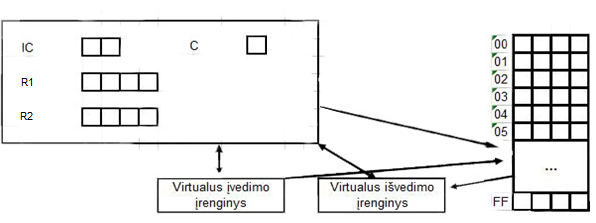
\includegraphics{VM.PNG}

\subsection{Virtualios mašinos komponentų aprašymas}
\begin{description}
\item[Atmintis] \leavevmode 

Virtualios mašinos (VM) atmintis sudaryta iš 16 žodžių po 4 baitus. 16 žodžių sudarys bloką. Kiekvienai VM skiriama po 16 blokų. Tuose šešiolikoje blokų turi tilpti programa.
Pirmuose keturiuose blokuose bus saugomos programos komandos, o likusiuose dvylika – programos darbui reikalingi duomenys.
Ryšiai tarp realaus ir virtualaus adrZeso bus nusakomi per puslapiavimo mechanizmą. Puslapiavimo lentelė bus saugoma paskutiniuose penkiuose atminties blokuose.


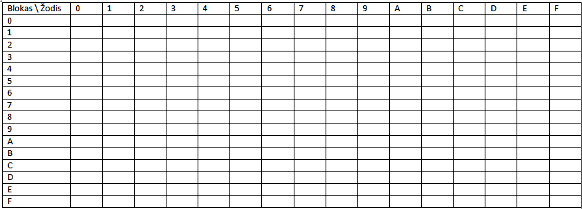
\includegraphics{VMatmintis.PNG}

\item[Procesorius]  \leavevmode 
  
Virtualios mašinos procesoriaus paskirtis – vykdyti programą, kuri yra virtualioje atmintyje. Kiekvienas procesas turi savo virtualų centrinį procesorių, tačiau sisteminių procesų programas vykdo aukšto lygio kalbos procesorius. 
Virtualaus procesoriaus registrai:
\begin{itemize}
\item R – 4 baitų bendro naudojimo registras;
\item D – 4 baitų bendro naudojimo registras;
\item IC – 2 baitų virtualios mašinos programos skaitiklis;
\item C – 1 baito loginis trigeris.
\end{itemize}
Galimos reikšmės:
\begin{itemize}
\item `T' - TRUE;
\item `F' – FALSE.
\end{itemize}  
  
\item[Komandų sistema] \leavevmode 
\begin{enumerate}
\item Aritmetinės komandos: \leavevmode 
\begin{itemize}
\item ADD – sudeda R1 ir R2, kur R1 ir R2 – įvedami skaičiai arba komandos, įrašoma į D3
\item SUB – iš R1 atimama R2, įrašoma į D3
\item MUL – sudaugina R1 ir R2, įrašoma į D3
\item DIV – padalina R1 iš R2, įrašoma į D3
\end{itemize}
\item Palyginimo komandos:
\begin{itemize}
\item CMP – ši komanda palygina registre R1 ir R2 išsaugoma į SF reikšmę: 0 – jei R1 = R2,  1 – jei R1 > R2, 2 –  R1 < R2.
\item JMP x1x2 - ši komanda pagal SF reikšmę „šoka“ į atminti su adresu 
\end{itemize}
\item  Darbo su duomenimis komandos:
\begin{itemize}
\item LDx1x2 – į registrą R1 užkrauna skaičių nurodytu adresu 16 * x1 + x2 bei formuoja SF = 4 požymį, reiškiantį, kad registre R1 – simbolinė informacija.
\item LWx1x2 – į registrą R1 užkrauna žodį nurodytu adresu 16 * x1 + x2 bei formuoja SF = 3 požymį, reškiantį, kad registre R1 – sveikas skaičius su ženklu.
\item LSx1x2 – į atmintį įkelia žodį ar skaičių.
\item LCx1x2 – iš realios atminties pasiima žodį ar skaičių ir įkelia į R1.
\item LEx1x2 – į registrą R2 užkrauna skaičių, adresu 16 * x1 + x2.
\item PD x1x2 – išvedimo komanda
\item LK x1x2 – nuskaito registrą R2
\end{itemize}
\item Valdymo komandos:
\begin{itemize}
\item JMx1x2 – besąlyginio valdymo perdavimo komanda. Ji reiškia, kad valdymas turi būti perduotas kodo segmento žodžiui, nurodytam adresu 16 * x1 + x2.
\item IC – komandos skaitliukas. IC = 16 * x1 + x2;
\item HALT – programos sustojimo taško komanda, t.y. programos valdymo pabaiga.
\end{itemize}
\end{enumerate}
\end{description}   
   
\subsection{Virtualios mašinos bendravimo su įvedimo/išvedimo įrenginiais
mechanizmo aprašymas}



\subsection{Virtualios mašinos interpretuojamojo vykdomojo failo išeities 
teksto formatas}

Užduoties kodas yra surašomas faile. Visame faile rašant tik vykdymui reikalingas
komandas. Paskutinė vykdoma komanda privalo būti HALT. Kitu atveju virtualios mašinos darbo
rezultatai nėra apibrėžti.

Bendra programos schema:\\
\\\textbf{DATASEG:}

DW simbolinis žodis – 4simboliai tarp kabučių (pvz.: DW "ABCD")

DPI neneigiamas sveikas skaičius (pvz. DPI 5)

DNI neigiamas sveikas skaičius (pvz. DNI -2)
\\\textbf{CODESEG:}

<komandos po 4 simbolius>\\
\textbf{HALT}

\subsection{Modeliuojamos virtualios mašinos loginių komponentų sąryšio su 
realios mašinos techninės įrangos komponentais aprašymas}

Sistemai aptikus pertraukimą, nutraukiamas vartotojo programos vykdymas, o valdymas perduodamas pertraukimo apdorojimo programai. Pastaroji programa, atlikusi darbą, valdymą grąžina operacinei sistemai pertraukimo vietoje.  Ką toliau daryti – sprendžia OS. Kiekvieno pertraukimą sukeliančio įvykio metu bus nustatomi atitinkami pertraukimų registrai: CH1, CH2, CH3, SI, PI, TIME priskiriamos atitinkamos reikšmės. 
Į pertraukimą reaguojama tik vartotojo režime, supervizoriaus režime pertraukimai uždrausti. Vykdant programas vartotojo režimu virtualioje mašinoje, vykdomas komandos interpretavimo ciklas ir po to duodama supervizorinė komanda Test(x), kuri  nustato ar neįvyko pertraukimas. 
Pertraukimui įvykus, išsaugoma virtualios mašinos būsena, procesorius perjungiamas į supervizoriaus režimą ir valdymas atiduodamas atitinkamo pertraukimo apdorojimo programai.
Pertraukimo programos nustato pertraukimą sukėlusią priežastį ir išvalo pertraukimo registrą, kviesdama komanda Test su atitinkamu parametru. Po  to reaguojant į pertraukimą.
Bendra taisyklė pertraukimų programų bendravimui su likusia sistemos dalimi tūrėtų būti tokia: duomenimis keičiamasi ne tiesiogiai, o per sutartus kintamuosius supervizorinėje atmintyje, kurių adresai yra iš anksto žinomi ir nesikeičia. Tai būtina, norint maksimaliai atriboti žemo lygio pertraukimų apdorojimo aparatūra nuo aukšto lygio operacinės sistemos.
   
%Visi skaičiai yra su ženklu!

%Komandų argumentai nurodyti 16-ainiais skaičiais.
